% XeLaTeX document
\documentclass[12pt,a4paper]{article}

% Редактируем: конфигурация, личные настройки: имя, название предмета и пр. для титульной страницы и метаданных документа здесь
\newcommand{\university}{Национальный исследовательский Университет ИТМО}
\newcommand{\mfaculty}{Мегафакультет информационных и трансляционных технологий}
\newcommand{\faculty}{Факультет инфокоммуникационных технологий}
\newcommand{\city}{Санкт-Петербург}
\newcommand{\num}{ №1}
\newcommand{\docname}{Лабораторная работа}
\newcommand{\subject}{Инфокоммуникационные технологии}
\newcommand{\tutorname}{О.М. Ромакина}
\newcommand{\studentname}{И.А. Абдулов}
\newcommand{\group}{K3121}

% Не редактируем: используемые пакеты
% настройка кодировки, шрифтов и русского языка
\usepackage{fontspec}
\usepackage{polyglossia}

% рабочие ссылки в документе
\usepackage{hyperref}

% графика
\usepackage{graphicx}
\usepackage{tikz}

% поворот страницы
\usepackage{pdflscape}

% качественные листинги кода
\usepackage{minted}
\usepackage{listings}
\usepackage{lstfiracode}

% отключение копирования номеров строк из листинга, работает не во всех просмотрщиках (в Adobe Reader работает)
\usepackage{accsupp}
\newcommand\emptyaccsupp[1]{\BeginAccSupp{ActualText={}}#1\EndAccSupp{}}
\let\theHFancyVerbLine\theFancyVerbLine
\def\theFancyVerbLine{\rmfamily\tiny\emptyaccsupp{\arabic{FancyVerbLine}}}

% библиография
\bibliographystyle{templates/gost-numeric.bbx}
\usepackage{csquotes}
\usepackage[parentracker=true,backend=biber,hyperref=true,bibencoding=utf8,style=numeric-comp,language=auto,autolang=other,citestyle=gost-numeric,defernumbers=true,bibstyle=gost-numeric,sorting=ntvy]{biblatex}

% установка полей
\usepackage{geometry}

% нумерация картинок по секциям
\usepackage{chngcntr}

% дополнительные команды для таблиц
\usepackage{booktabs}

% для заголовков
\usepackage{caption}
\usepackage{titlesec}
\usepackage[dotinlabels]{titletoc}

% разное для математики
\usepackage{amsmath, amsfonts, amssymb, amsthm, mathtools}

% водяной знак на документе, см. main.tex
\usepackage[printwatermark]{xwatermark}


% Не редактируем: параметры используемых пакетов и не только
% настройки polyglossia
\setdefaultlanguage{russian}
\setotherlanguage{english}

% локализация
\addto\captionsrussian{
	\renewcommand{\figurename}{Рисунок}%
	\renewcommand{\partname}{Глава}
	\renewcommand{\contentsname}{\centerline{Содержание}}
	\renewcommand{\listingscaption}{Листинг}
}

% основной шрифт документа
\setmainfont{CMU Serif}
\newfontfamily\cyrillicfont{CMU Serif}[Script=Cyrillic]

% перечень использованных источников
\addbibresource{refs.bib}

% настройка полей
\geometry{top=2cm}
\geometry{bottom=2cm}
\geometry{left=2cm}
\geometry{right=2cm}
\geometry{bindingoffset=0cm}

% настройка ссылок и метаданных документа
\hypersetup{unicode=true,colorlinks=true,linkcolor=red,citecolor=green,filecolor=magenta,urlcolor=cyan,
	pdftitle={\docname},
	pdfauthor={\studentname},
	pdfsubject={\subject},
	pdfcreator={\studentname},
	pdfproducer={Overleaf},
	pdfkeywords={\subject}
}

% настройка подсветки кода и окружения для листингов
\usemintedstyle{colorful}
\newenvironment{code}{\captionsetup{type=listing}}{}

% шрифт для листингов с лигатурами
\setmonofont{FiraCode-Regular.otf}[
	SizeFeatures={Size=10},
	Path = templates/,
	Contextuals=Alternate
]

% оформления подписи рисунка
\captionsetup[figure]{labelsep = period}

% подпись таблицы
\DeclareCaptionFormat{hfillstart}{\hfill#1#2#3\par}
\captionsetup[table]{format=hfillstart,labelsep=newline,justification=centering,skip=-10pt,textfont=bf}

% путь к каталогу с рисунками
\graphicspath{{fig/}}

% Внесение titlepage в учёт счётчика страниц
\makeatletter
\renewenvironment{titlepage} {
	\thispagestyle{empty}
}
\makeatother

\counterwithin{figure}{section}
\counterwithin{table}{section}

\titlelabel{\thetitle.\quad}

% для удобного конспектирования математики
\mathtoolsset{showonlyrefs=true}
\theoremstyle{plain}
\newtheorem{theorem}{Теорема}[section]
\newtheorem{proposition}[theorem]{Утверждение}
\newtheorem{lemma}[theorem]{Лемма}
\theoremstyle{definition}
\newtheorem{corollary}{Следствие}[theorem]
\newtheorem{problem}{Задача}[section]
\theoremstyle{remark}
\newtheorem*{nonum}{Решение}

% настоящее матожидание
\newcommand{\MExpect}{\mathsf{M}}

% объявили оператор!
\DeclareMathOperator{\sgn}{\mathop{sgn}}

% перенос знаков в формулах (по Львовскому)
\newcommand*{\hm}[1]{#1\nobreak\discretionary{} {\hbox{$\mathsurround=0pt #1$}}{}}


% водяной знак для обозначения статуса документа
%\newwatermark[allpages,color=red!5,angle=45,scale=3,xpos=0,ypos=0]{DRAFT}
\begin{document}
% Не редактируем: Титульная страница (формируется автоматически из заданной конфигурации)
\begin{titlepage}	% начало титульной страницы

	\begin{center}		% выравнивание по центру

		\large \university \\
		\large \mfaculty \\
		\large \faculty \\[6cm]
		% название института, затем отступ 6см

		\huge \subject \\[0.5cm] % название работы, затем отступ 0,5см
		\large \docname  \num \\[5.1cm]
		 %\large Разработка методов обучения с подкреплением\\[5cm]

	\end{center}


	\begin{flushright} % выравнивание по правому краю
		\begin{minipage}{0.25\textwidth} % врезка в половину ширины текста
			\begin{flushleft} % выровнять её содержимое по левому краю

				\large\textbf{Работу выполнил:}\\
				\large \studentname \\
				\large {Группа:} \group \\

				\large \textbf{Преподаватель:}\\
				\large \tutorname

			\end{flushleft}
		\end{minipage}
	\end{flushright}

	\vfill % заполнить всё доступное ниже пространство

	\begin{center}
		\large \city \\
		\large \the\year % вывести дату
	\end{center} % закончить выравнивание по центру

\end{titlepage} % конец титульной страницы

\vfill % заполнить всё доступное ниже пространство


% Не редактируем: Страница содержания (формируется автоматически из section, subsection и пр., указанных в content.tex)
% Содержание
\tableofcontents
\newpage



% Редактируем: всё остальное: вступление, др. этапы, заключение, приложение
\section*{Введение}

Лабораторная работа актуальна, потому что в ней студент учится использовать текстовый редактор \LaTeX\ для написания отчета по лабораторной работе, которая содержит много математического текста из учебника по матанализу\cite{matan}, а также рисунки / формулы / таблицы согласно приведенному шаблону.

\addcontentsline{toc}{section}{Введение}

\newpage
\section{Функция}

\subsection{Простейшая классификация отображений}

Когда функцию $f\colon \mathbb{X} \to \mathbb{Y}$ называют отображением, значение $f(x) \in \mathbb{Y}$, которое она принимает на элементе $x \in \mathbb{X}$, обычно называют образом элемента $x$.

Образом множества $\mathbb{A} \subset \mathbb{X}$ при отображении $f\colon \mathbb{\mathbb{X}} \to \mathbb{Y}$ называют множество (см. \eqref{eq:1})
\begin{equation}
\label{eq:1}
    f(\mathbb{A}) := \{y \in \mathbb{Y} \mid \exists x \ ((x \in \mathbb{A})\land(y=f(x)))\} 
\end{equation}
тех элементов $\mathbb{Y}$, которые являются образами элементов множества $\mathbb{A}$.


Множество (см. \eqref{eq:2})
\begin{equation}
\label{eq:2}
f^{-1}(\mathbb{B}) := \{ x \in \mathbb{X} \lor f(x) \in \mathbb{B}\}
\end{equation}
тех элементов $\mathbb{X}$, образы которых содержатся в $\mathbb{B}$, называют прообразом (или
полным прообразом) множества $\mathbb{B} \subset \mathbb{Y}$ (Рисунок~\ref{pic:pic1}).

\begin{figure}[H]
	\begin{center}
		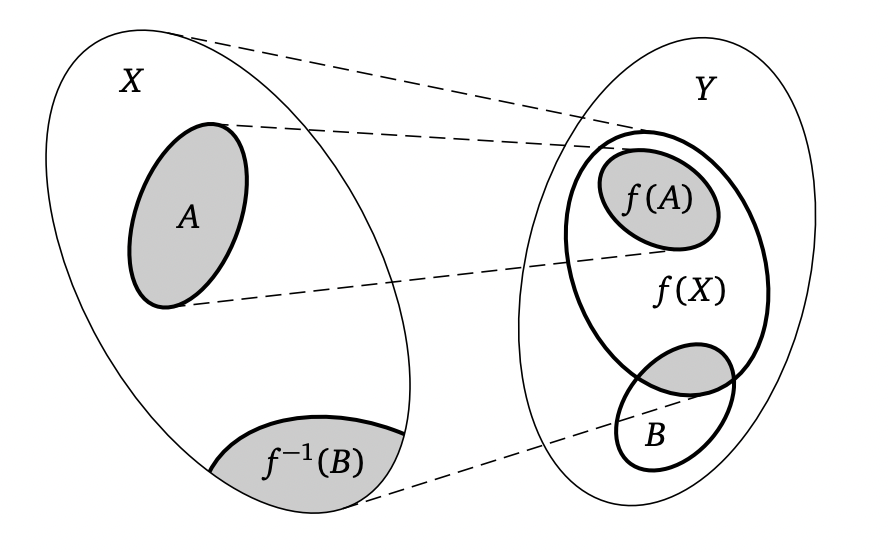
\includegraphics[scale=0.7]{pic1.png}
		\caption{Образы и прообразы}
		\label{pic:pic1} % название для ссылок внутри кода
	\end{center}
\end{figure}

Про отображение $f\colon \mathbb{X} \to \mathbb{Y}$ говорят, что оно

сюръективно (или есть отображение $\mathbb{X}$ на $\mathbb{Y}$), если $f(\mathbb{X})=\mathbb{Y}$;

инъективно \eqref{eq:3} (или есть вложение, инъекция), если для любых элементов $x_1$, $x_2$ множества $\mathbb{X}$

\begin{equation}
\label{eq:3}
(f(x_1)=f(x_2)) \Rightarrow (x_1=x_2),
\end{equation}
т. е. различные элементы имеют различные образы;

биективно (или взаимно однозначно), если оно сюръективно и инъективно одновременно.

Если отображение $f\colon \mathbb{X} \to \mathbb{Y}$ биективно, т. е. является взаимно однозначным соответствием между элементами множеств $\mathbb{X}$ и $\mathbb{Y}$, то естественно возникает отображение \eqref{eq:4}
\begin{equation}
\label{eq:4}
f^{-1}\colon \mathbb{Y} \to \mathbb{X},
\end{equation}
которое определяется следующим образом: если $f(x)=y$, то $f^{-1}(y)=x$, т. е.
элементу $y \in \mathbb{Y}$ ставится в соответствие тот элемент $x \in \mathbb{X}$, образом которого при отображении $f$ является $y$. В силу сюръективности $f$ такой элемент
$x \in \mathbb{X}$ найдется, а ввиду инъективности $f$ он единственный. Таким образом,
отображение $f^{-1}$ определено корректно. Это отображение называют обратным по отношению к исходному отображению $f$.

Из построения обратного отображения видно, что $f^{-1}\colon \mathbb{Y} \to \mathbb{X}$ само является биективным и что обратное к нему отображение $(f^{-1})^{-1}\colon \mathbb{Y} \to \mathbb{X}$ совпадает с $f\colon \mathbb{X} \to \mathbb{Y}$.

Таким образом, свойство двух отображений быть обратными является
взаимным: если $f^{-1}$ — обратное для $f$, то, в свою очередь, $f$ — обратное
для $f^{-1}$.

Заметим, что символ $f^{-1}(\mathbb{B})$ прообраза множества $\mathbb{B} \subset \mathbb{Y}$ ассоциируется с
символом $f^{-1}$ обратной функции, однако следует иметь в виду, что прообраз
множества определен для любого отображения $f\colon \mathbb{X} \to \mathbb{Y}$, даже если оно не
является биективным и, следовательно, не имеет обратного.

\begin{table}[H]
	\caption{Виды отображений}
	\begin{center}
		\begin{tabular}{p{0.3\textwidth}p{0.3\textwidth}p{0.3\textwidth}}
			\toprule
			Сюръективное & Инъективное & Биективное \\
			\midrule
			каждый элемент множества $\mathbb{X}$ является образом хотя бы одного элемента из множества $\mathbb{Y}$           & каждый элемент множества $\mathbb{Y}$ является образом не более 1 элемента из $\mathbb{X}$          & сюръективно и инъективно одновременно \\

            $\forall y \in \mathbb{Y}\ \exists x \in \mathbb{X}\colon y = \varphi(x)$       & $\varphi(x)=\varphi(y)\Rightarrow x=y$    & $\varphi\colon \mathbb{X}\leftrightarrow \mathbb{Y}$ \\
			
			\bottomrule
            
		\end{tabular}
		\label{tabular:tab1}
	\end{center}
\end{table}

\subsection{Композиция функций и взаимно обратные отображения}
Богатым источником новых функций, с одной стороны, и способом расчленения сложных функций на более простые — с другой, является операция композиции
отображений.

Если отображения $f\colon \mathbb{X} \to \mathbb{Y}$ и $g\colon \mathbb{Y} \to \mathbb{Z}$ таковы, что одно из них (в нашем
случае $g$) определено на множестве значений другого ($f$), то можно построить новое отображение \eqref{eq:5}
\begin{equation}
\label{eq:5}
g \circ f\colon \mathbb{X} \to \mathbb{Z},
\end{equation}
значения которого на элементах множества $\mathbb{X}$ определяются формулой \eqref{eq:6}
\begin{equation}
\label{eq:6}
(g \circ f)(x) := g(f(x)).
\end{equation}

Построенное составное отображение $g \circ f$ называют композицией отображения $f$ и отображения $g$ (в таком порядке!).

\begin{figure}[H]
	\begin{center}
		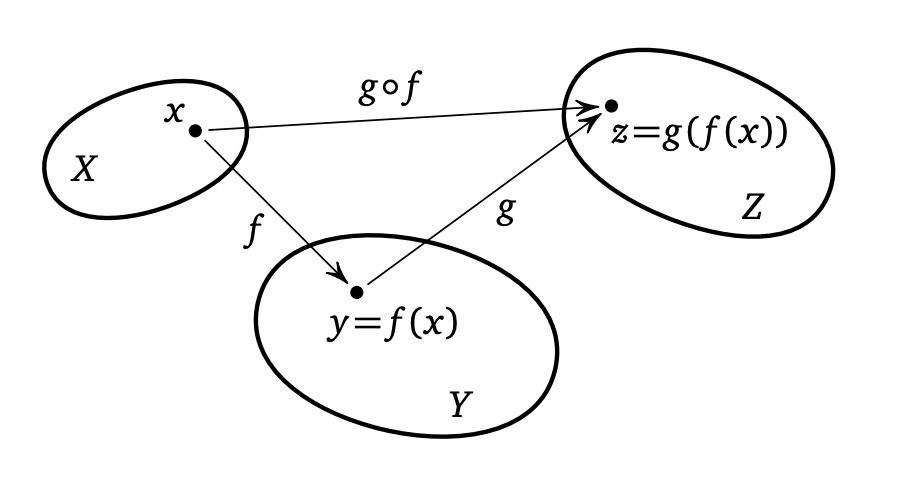
\includegraphics[scale=0.7]{pic2.png}
		\caption{Конструкция композиции отображений $f$ и $g$}
		\label{pic:pic2} % название для ссылок внутри кода
	\end{center}
\end{figure}

С композицией отображений вы уже неоднократно встречались как в геометрии, рассматривая композицию движений плоскости или пространства,
так и в алгебре при исследовании «сложных» функций, полученных композицией простейших элементарных функций.

Операцию композиции иногда приходится проводить несколько раз подряд, и в этой связи полезно отметить, что она ассоциативна, т. е. выполняется \eqref{eq:7}
\begin{equation}
\label{eq:7}
h \circ (g \circ f)=(h \circ g) \circ f
\end{equation}

Действительно \eqref{eq:8},
\begin{equation}
\label{eq:8}
h \circ (g \circ f)(x)=h((g \circ f)(x))=(h \circ g)(f(x))=((h \circ g) \circ f)(x).
\end{equation}

Это обстоятельство, как и в случае сложения или умножения нескольких
чисел, позволяет опускать скобки, предписывающие порядок спаривания.

Если в композиции $f_n \circ \dots \circ f_1$ все члены одинаковы и равны $f$, то ее обозначают коротко $f^n$.

Хорошо известно, например, что корень квадратный из положительного
числа $a$ можно вычислить последовательными приближениями по формуле \eqref{eq:9}
\begin{equation}
\label{eq:9}
x_{n+1}=\frac{1}{2} (x_n + \frac{a}{x_n}),
\end{equation}
начиная с любого начального приближения $x_0>0$. Это не что иное, как последовательное вычисление $f^n(x_0)$, где $f(x)=\frac{1}{2}(x+\frac{a}{x})$. Такая процедура, когда вычисленное на предыдущем шаге значение функции на следующем
шаге становится ее аргументом, называется итерационным процессом. Итерационные процессы широко используются в математике.

Отметим также, что даже в том случае, когда обе композиции $g \circ f$ и $f \circ g$
определены, вообще говоря \eqref{eq:10},
\begin{equation}
\label{eq:10}
g \circ f \ne f \circ g.
\end{equation}

Действительно, возьмем, например, двухэлементное множество $\{a, b\}$ и
отображения $f \colon \{a, b\} \to a, g \colon \{a, b\} \to b$. Тогда, очевидно, $g \circ f \colon \{a, b\} \to b$, в то время как $f \circ g \colon \{a, b\} \to a$.

Отображение $f \colon \mathbb{X} \to \mathbb{X}$, сопоставляющее каждому элементу множества $\mathbb{X}$
его самого, т. е. $x \xrightarrow{f} x$, будем обозначать через $e_x$ и называть тождественным отображением множества $\mathbb{X}$.

\begin{lemma}

\begin{equation}
	(g \circ f=e_x) \Rightarrow (g \text{ сюръективно})\land(f \text{ инъективно}).
\end{equation}

\begin{proof} Если $f \colon \mathbb{X} \to \mathbb{Y}$, $g \colon \mathbb{Y} \to \mathbb{X}$ и $g \circ f=e_\mathbb{X} \colon \mathbb{X} \to \mathbb{X}$, то
\begin{equation}
\mathbb{X}=e_\mathbb{X}(\mathbb{X})=(g \circ f)(\mathbb{X})=g(f(\mathbb{X})) \subset g(\mathbb{Y})
\end{equation}
и, значит, $g$ сюръективно.

Далее, если $x_1 \in \mathbb{X}$ и $x_2 \in \mathbb{X}$, то
\begin{multline}
(x_1 \ne x_2) \Rightarrow (e_\mathbb{X}(x_1) \ne e_\mathbb{X}(x_2)) \Rightarrow ((g \circ f)(x_1) \ne (g \circ f)(x_2)) \Rightarrow \\
\Rightarrow g(f(x_1)) \ne g(f(x_2)) \Rightarrow (f(x_1) \ne f(x_2)),
\end{multline}
следовательно, $f$ инъективно.
\end{proof}
\end{lemma}

Через операцию композиции отображений можно описать взаимно обратные отображения.
\begin{proposition}
Отображения $f \colon \mathbb{X} \to \mathbb{Y}$, $g \colon \mathbb{Y} \to \mathbb{X}$ являются биективными и взаимно обратными в том и только в том случае, когда $g \circ f=e_\mathbb{X}$ и $f \circ g=e_\mathbb{Y}$.
\end{proposition}
\begin{proof}
В силу леммы одновременное выполнение условий $g \circ f=e_\mathbb{X}$ и $f \circ g=e_\mathbb{Y}$ гарантирует сюръективность и инъективность, т. е. биективность каждого
из отображений $f$, $g$.

Эти же условия показывают, что $y=f(x)$ в том и только в том случае, когда $x=g(y)$.
\end{proof}
Выше мы исходили из явного построения обратного отображения. Из доказанного утверждения следует, что мы могли бы дать менее наглядное, но
зато более симметричное определение взаимно обратных отображений как
таких, которые удовлетворяют двум условиям: $g \circ f=e_\mathbb{X}$ и $f \circ g=e_\mathbb{Y}$.

\newpage
\section*{Заключение}
\LaTeX\ удобен для создания отчётов, так как сам следит за нумерацией таблиц, рисунков, листингов и отсылок к ним (так, например, здесь всегда будет указан номер рисунка "Конструкция композиции отображений $f$ и $g$" не зависимо от того, какой он (1,2 или другой) - это рисунок \ref{pic:pic2}). Не менее важно что весь документ оформлен в едином стиле, а исходные материалы подключаются к отчёту, а не хранятся в нём. Всё это позволяет легко получить качественный отчёт без дополнительных трат на его офрмление.

Исключения, пожалуй, составляют таблицы, так как их значительно сложнее создавать кодом, нежели в графическом редакторе. Но здесь никто не запрещает использовать визуальные средства создания таблиц для \LaTeX.
\addcontentsline{toc}{section}{Заключение}


% Не редактируем: Страница библиографии (формируется автоматически из книжек, указанных в refs.bib и пометок \cite{имя_источника} в тексте)
\newpage
\printbibliography[title=Список использованных источников]
\addcontentsline{toc}{section}{Список использованных источников}
\end{document}
